% Options for packages loaded elsewhere
\PassOptionsToPackage{unicode}{hyperref}
\PassOptionsToPackage{hyphens}{url}
%
\documentclass[
]{book}
\usepackage{amsmath,amssymb}
\usepackage{lmodern}
\usepackage{iftex}
\ifPDFTeX
  \usepackage[T1]{fontenc}
  \usepackage[utf8]{inputenc}
  \usepackage{textcomp} % provide euro and other symbols
\else % if luatex or xetex
  \usepackage{unicode-math}
  \defaultfontfeatures{Scale=MatchLowercase}
  \defaultfontfeatures[\rmfamily]{Ligatures=TeX,Scale=1}
\fi
% Use upquote if available, for straight quotes in verbatim environments
\IfFileExists{upquote.sty}{\usepackage{upquote}}{}
\IfFileExists{microtype.sty}{% use microtype if available
  \usepackage[]{microtype}
  \UseMicrotypeSet[protrusion]{basicmath} % disable protrusion for tt fonts
}{}
\makeatletter
\@ifundefined{KOMAClassName}{% if non-KOMA class
  \IfFileExists{parskip.sty}{%
    \usepackage{parskip}
  }{% else
    \setlength{\parindent}{0pt}
    \setlength{\parskip}{6pt plus 2pt minus 1pt}}
}{% if KOMA class
  \KOMAoptions{parskip=half}}
\makeatother
\usepackage{xcolor}
\usepackage{color}
\usepackage{fancyvrb}
\newcommand{\VerbBar}{|}
\newcommand{\VERB}{\Verb[commandchars=\\\{\}]}
\DefineVerbatimEnvironment{Highlighting}{Verbatim}{commandchars=\\\{\}}
% Add ',fontsize=\small' for more characters per line
\usepackage{framed}
\definecolor{shadecolor}{RGB}{248,248,248}
\newenvironment{Shaded}{\begin{snugshade}}{\end{snugshade}}
\newcommand{\AlertTok}[1]{\textcolor[rgb]{0.94,0.16,0.16}{#1}}
\newcommand{\AnnotationTok}[1]{\textcolor[rgb]{0.56,0.35,0.01}{\textbf{\textit{#1}}}}
\newcommand{\AttributeTok}[1]{\textcolor[rgb]{0.77,0.63,0.00}{#1}}
\newcommand{\BaseNTok}[1]{\textcolor[rgb]{0.00,0.00,0.81}{#1}}
\newcommand{\BuiltInTok}[1]{#1}
\newcommand{\CharTok}[1]{\textcolor[rgb]{0.31,0.60,0.02}{#1}}
\newcommand{\CommentTok}[1]{\textcolor[rgb]{0.56,0.35,0.01}{\textit{#1}}}
\newcommand{\CommentVarTok}[1]{\textcolor[rgb]{0.56,0.35,0.01}{\textbf{\textit{#1}}}}
\newcommand{\ConstantTok}[1]{\textcolor[rgb]{0.00,0.00,0.00}{#1}}
\newcommand{\ControlFlowTok}[1]{\textcolor[rgb]{0.13,0.29,0.53}{\textbf{#1}}}
\newcommand{\DataTypeTok}[1]{\textcolor[rgb]{0.13,0.29,0.53}{#1}}
\newcommand{\DecValTok}[1]{\textcolor[rgb]{0.00,0.00,0.81}{#1}}
\newcommand{\DocumentationTok}[1]{\textcolor[rgb]{0.56,0.35,0.01}{\textbf{\textit{#1}}}}
\newcommand{\ErrorTok}[1]{\textcolor[rgb]{0.64,0.00,0.00}{\textbf{#1}}}
\newcommand{\ExtensionTok}[1]{#1}
\newcommand{\FloatTok}[1]{\textcolor[rgb]{0.00,0.00,0.81}{#1}}
\newcommand{\FunctionTok}[1]{\textcolor[rgb]{0.00,0.00,0.00}{#1}}
\newcommand{\ImportTok}[1]{#1}
\newcommand{\InformationTok}[1]{\textcolor[rgb]{0.56,0.35,0.01}{\textbf{\textit{#1}}}}
\newcommand{\KeywordTok}[1]{\textcolor[rgb]{0.13,0.29,0.53}{\textbf{#1}}}
\newcommand{\NormalTok}[1]{#1}
\newcommand{\OperatorTok}[1]{\textcolor[rgb]{0.81,0.36,0.00}{\textbf{#1}}}
\newcommand{\OtherTok}[1]{\textcolor[rgb]{0.56,0.35,0.01}{#1}}
\newcommand{\PreprocessorTok}[1]{\textcolor[rgb]{0.56,0.35,0.01}{\textit{#1}}}
\newcommand{\RegionMarkerTok}[1]{#1}
\newcommand{\SpecialCharTok}[1]{\textcolor[rgb]{0.00,0.00,0.00}{#1}}
\newcommand{\SpecialStringTok}[1]{\textcolor[rgb]{0.31,0.60,0.02}{#1}}
\newcommand{\StringTok}[1]{\textcolor[rgb]{0.31,0.60,0.02}{#1}}
\newcommand{\VariableTok}[1]{\textcolor[rgb]{0.00,0.00,0.00}{#1}}
\newcommand{\VerbatimStringTok}[1]{\textcolor[rgb]{0.31,0.60,0.02}{#1}}
\newcommand{\WarningTok}[1]{\textcolor[rgb]{0.56,0.35,0.01}{\textbf{\textit{#1}}}}
\usepackage{longtable,booktabs,array}
\usepackage{calc} % for calculating minipage widths
% Correct order of tables after \paragraph or \subparagraph
\usepackage{etoolbox}
\makeatletter
\patchcmd\longtable{\par}{\if@noskipsec\mbox{}\fi\par}{}{}
\makeatother
% Allow footnotes in longtable head/foot
\IfFileExists{footnotehyper.sty}{\usepackage{footnotehyper}}{\usepackage{footnote}}
\makesavenoteenv{longtable}
\usepackage{graphicx}
\makeatletter
\def\maxwidth{\ifdim\Gin@nat@width>\linewidth\linewidth\else\Gin@nat@width\fi}
\def\maxheight{\ifdim\Gin@nat@height>\textheight\textheight\else\Gin@nat@height\fi}
\makeatother
% Scale images if necessary, so that they will not overflow the page
% margins by default, and it is still possible to overwrite the defaults
% using explicit options in \includegraphics[width, height, ...]{}
\setkeys{Gin}{width=\maxwidth,height=\maxheight,keepaspectratio}
% Set default figure placement to htbp
\makeatletter
\def\fps@figure{htbp}
\makeatother
\setlength{\emergencystretch}{3em} % prevent overfull lines
\providecommand{\tightlist}{%
  \setlength{\itemsep}{0pt}\setlength{\parskip}{0pt}}
\setcounter{secnumdepth}{5}
\usepackage{booktabs}
\ifLuaTeX
  \usepackage{selnolig}  % disable illegal ligatures
\fi
\usepackage[]{natbib}
\bibliographystyle{plainnat}
\IfFileExists{bookmark.sty}{\usepackage{bookmark}}{\usepackage{hyperref}}
\IfFileExists{xurl.sty}{\usepackage{xurl}}{} % add URL line breaks if available
\urlstyle{same} % disable monospaced font for URLs
\hypersetup{
  pdftitle={AIS: Capacitación de R},
  pdfauthor={Oliab Herrera Coria},
  hidelinks,
  pdfcreator={LaTeX via pandoc}}

\title{AIS: Capacitación de R}
\author{Oliab Herrera Coria}
\date{2023-02-09}

\begin{document}
\maketitle

{
\setcounter{tocdepth}{1}
\tableofcontents
}
\hypertarget{informaciuxf3n-del-curso}{%
\chapter*{Información del curso}\label{informaciuxf3n-del-curso}}
\addcontentsline{toc}{chapter}{Información del curso}

\begin{itemize}
\item
  Este es un curso de Introducción a R.
\item
  Al final serán capaces de utilizar R para cargar datos, arreglarlos, hacer gráficos y tablas, e informes en Rmarkdown.
\item
  Intentaremos que el curso sea fundamentalmente práctico.
\item
  En lugar de presentar todos los pormenores de R de manera lineal, se irán presentando distintos aspectos de R conforme se vayan necesitando; es decir, no vamos a presentar R como un lenguaje de programación sino como una herramienta para hacer análisis estadísticos.
\end{itemize}

E- n la carpeta del curso están todos los materiales: tutoriales, algunos datos, etc\ldots.

\hypertarget{ligas}{%
\subsubsection*{Ligas}\label{ligas}}
\addcontentsline{toc}{subsubsection}{Ligas}

Notas: \url{https://fastidious-brioche-36f6dd.netlify.app/}
Correo: \href{mailto:oliabherrera@gmail.com}{\nolinkurl{oliabherrera@gmail.com}}

\hypertarget{temario}{%
\section*{Temario}\label{temario}}
\addcontentsline{toc}{section}{Temario}

\begin{enumerate}
\def\labelenumi{\arabic{enumi}.}
\tightlist
\item
  \textbf{Introducción a R}
\end{enumerate}

\begin{itemize}
\tightlist
\item
  Instalación de R y R Studio.
\item
  Entorno de trabajo de RStudio.
\item
  Instalación de paquetes.
\item
  Ayuda en R.
\end{itemize}

\begin{enumerate}
\def\labelenumi{\arabic{enumi}.}
\setcounter{enumi}{1}
\tightlist
\item
  \textbf{Manipulación y visualización de datos}
\end{enumerate}

\begin{itemize}
\tightlist
\item
  Comandos básicos de R.
\item
  Manipulación y limpieza de datos.
\item
  Visualización de datos.
\item
  Temas selectos de programación en R.
\end{itemize}

\begin{enumerate}
\def\labelenumi{\arabic{enumi}.}
\setcounter{enumi}{2}
\tightlist
\item
  \textbf{Reportes POS}
\end{enumerate}

\begin{itemize}
\tightlist
\item
  Descarga de datos.
\item
  Scripts principales.
\item
  Proyecciones.
\end{itemize}

\hypertarget{software}{%
\subsection*{Software}\label{software}}
\addcontentsline{toc}{subsection}{Software}

\begin{itemize}
\tightlist
\item
  \url{https://www.r-project.org}
\item
  \url{https://www.rstudio.com}
\end{itemize}

\hypertarget{introducciuxf3n-a-r.}{%
\chapter{Introducción a R.}\label{introducciuxf3n-a-r.}}

El objetivo de este tutorial es familiarizarnos con el entorno de trabajo que proporciona R y RStudio. Al finalizar este tutorial también deberemos ser capaces de instalar y cargar los paquetes que vayamos a necesitar para realizar nuestros análisis de datos.

\hypertarget{instalaciuxf3n-de-r-y-r-studio.}{%
\section{Instalación de R y R Studio.}\label{instalaciuxf3n-de-r-y-r-studio.}}

Para instalar R vamos a la página web de R project: \url{http://www.r-project.org}

\begin{figure}
\centering
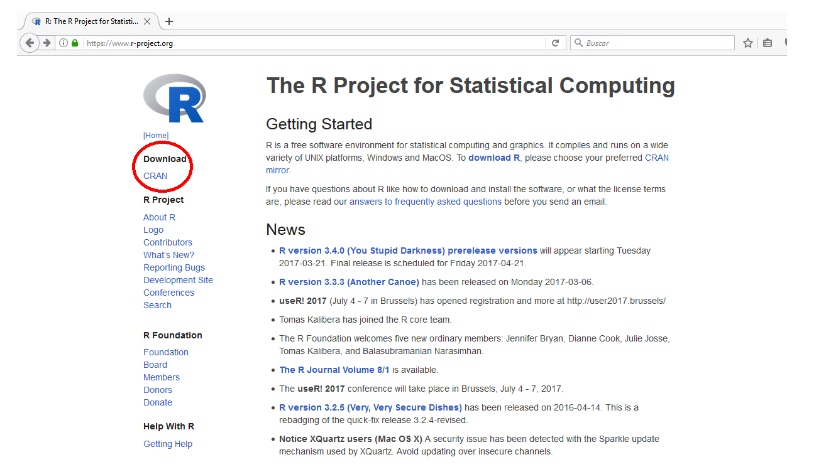
\includegraphics{imagenes/01.png}
\caption{Figura 1}
\end{figure}

Para descargar la aplicación hacemos clic en Cran y pinchamos sobre el enlace del ``espejo'' más próximo a nuestra ubicación, México. Seleccionemos la URL de, por ejemplo (\url{https://cran.itam.mx/}).

\begin{figure}
\centering
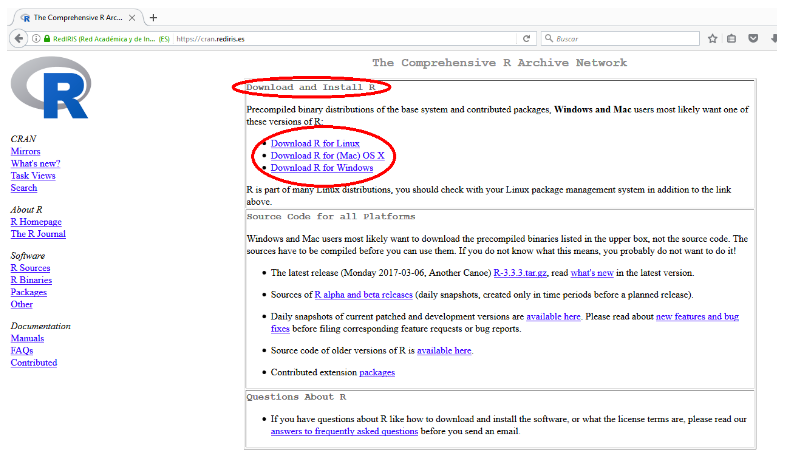
\includegraphics{imagenes/02.png}
\caption{Figura 2}
\end{figure}

Ahora, en función del tu sistema operativo, seleccionar la correspondiente opción.

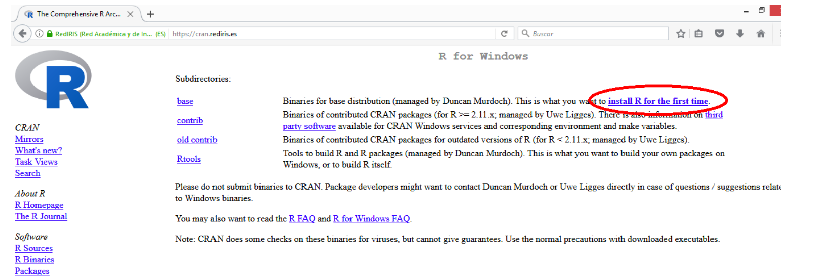
\includegraphics{imagenes/03.png}
\#\#\# Instalar R en Windows.

Al hacer clic sobre Download R for Windows iremos a la página que se reproduce más abajo. Hacer clic sobre \emph{install R for the first time.}

En la siguiente ventana, hacer clic sobre \emph{Download R 3.3.3 for Windows} y guardar el archivo de instalación.

Ejecutar el archivo descargado para proceder a la instalación de R.

\hypertarget{instalar-r-en-mac.}{%
\subsection{Instalar R en Mac.}\label{instalar-r-en-mac.}}

Al hacer clic sobre Download R for (Mac) OS X iremos a la página que se reproduce más abajo. Hacer clic sobre install R for the first time.

\begin{figure}
\centering
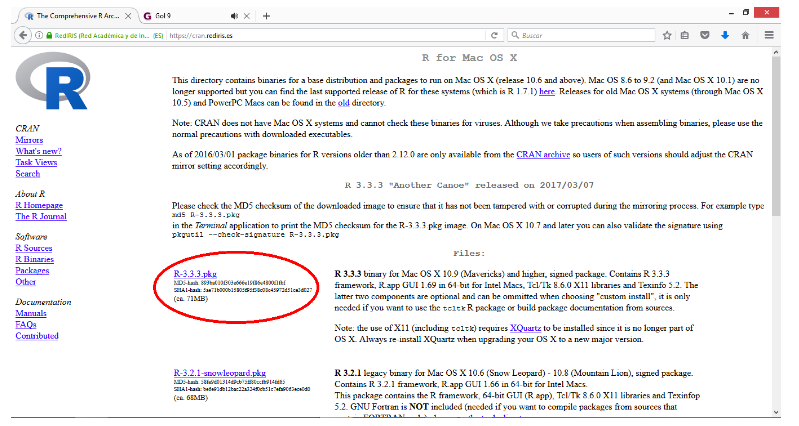
\includegraphics{imagenes/04.png}
\caption{Figura 4}
\end{figure}

Hacer clic sobre R-3.3.3.pkg y guardar el archivo de instalación. Ejecutar el archivo descargado para proceder a la instalación de R.

\hypertarget{instalar-rstudio}{%
\subsection{Instalar RStudio}\label{instalar-rstudio}}

Descargamos la aplicación desde la página web de RStudio \href{https://posit.co/download/rstudio-desktop/}{aquí} según nuestra plataforma de trabajo:

\begin{itemize}
\item
  RStudio 1.0.136 - Windows Vista/7/8/10.
\item
  RStudio 1.0.136 - Mac OS X 10.6+ (64-bit).
\end{itemize}

Una vez guardado el archivo, lo ejecutamos para instalar RStudio. Sigue las instrucciones de instalación.

\hypertarget{entorno-de-trabajo-de-rstudio.}{%
\section{Entorno de trabajo de RStudio.}\label{entorno-de-trabajo-de-rstudio.}}

En general trabajamos con la interfaz de RStudio antes que con la de R porque la primera es ``más amigable''.

Si abrimos RStudio vamos a ver algo parecido a lo que se muestra en la siguiente imagen:

\begin{figure}
\centering
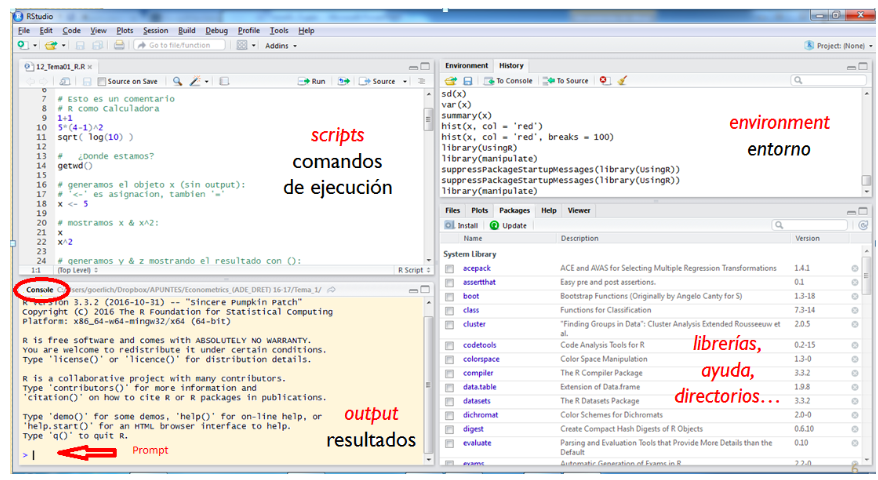
\includegraphics{imagenes/05.png}
\caption{Figura 5}
\end{figure}

Una vez estamos en RStudio, podemos escribir y ejecutar las órdenes de varias formas:

\begin{itemize}
\item
  directamente en la consola.
\item
  a través de un script (.R).
\item
  con ficheros Rmarkdown (.Rmd).
\end{itemize}

Como podemos ver, RStudio está (normalmente) dividido en 4 paneles.

\hypertarget{consola}{%
\subsection{Consola}\label{consola}}

Por defecto, la consola se encuentra en el panel inferior-izquierdo. ¿Vemos la pestaña que pone Console? Inmediatamente debajo aparece un texto informativo y, finalmente, el símbolo ``\textgreater{}''. Aquí es donde R espera que le demos instrucciones. Para ejecutarlas y obtener el resultado pulsamos enter.

Vamos a hacer este ejemplo:

\begin{Shaded}
\begin{Highlighting}[]
\DecValTok{2}\SpecialCharTok{+}\DecValTok{2}
\end{Highlighting}
\end{Shaded}

\begin{verbatim}
## [1] 4
\end{verbatim}

\begin{Shaded}
\begin{Highlighting}[]
\DecValTok{5}\SpecialCharTok{*}\NormalTok{(}\DecValTok{3{-}1}\NormalTok{)}\SpecialCharTok{\^{}}\DecValTok{2}
\end{Highlighting}
\end{Shaded}

\begin{verbatim}
## [1] 20
\end{verbatim}

\begin{Shaded}
\begin{Highlighting}[]
\FunctionTok{sqrt}\NormalTok{(}\DecValTok{4}\NormalTok{)}
\end{Highlighting}
\end{Shaded}

\begin{verbatim}
## [1] 2
\end{verbatim}

\hypertarget{scripts}{%
\subsection{Scripts}\label{scripts}}

Trabajar en la consola es muy limitado ya que las instrucciones se han de introducir una a una. Lo habitual es trabajar con scripts o ficheros de instrucciones. Estos ficheros tienen extensión \textbf{.R}.

Se puede crear una script con cualquier editor de texto (uno de los más populares es Tinn-R), pero nosotros lo haremos desde RStudio. Para ello, seleccionamos la siguiente ruta de menús: \textbf{File \textgreater{} New File \textgreater{} R script}

\begin{figure}
\centering
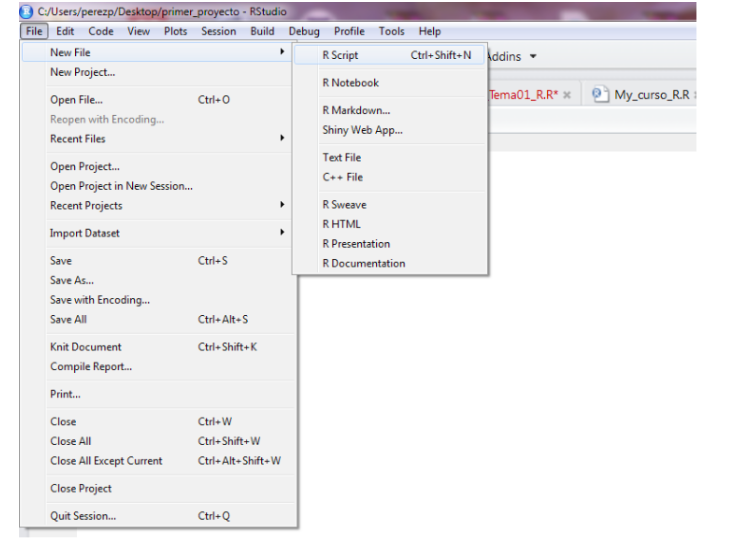
\includegraphics{imagenes/06.png}
\caption{Figura 5}
\end{figure}

El panel del script se sitúa en la parte superior-izquierda de RStudio. Ahora podemos escribir las instrucciones línea por línea. Las instrucciones las podemos ejecutar una a una o las podemos seleccionar y ejecutar en bloque. Para ejecutar las instrucciones tenemos varias alternativas:

\begin{itemize}
\item
  Hacemos clic en el botón: \textbf{Run} (botón situado en la parte derecha de las opciones del panel de script)
\item
  Pulsamos Ctrl+r
\item
  Ejecutamos el código desde las opciones del menú Code. Sinceramente, esto nunca lo hemos utilizado. ¡Cuestión de comodidad!
\end{itemize}

Como se muestra en la imagen más abajo, vamos a escribir nuestro primer script.

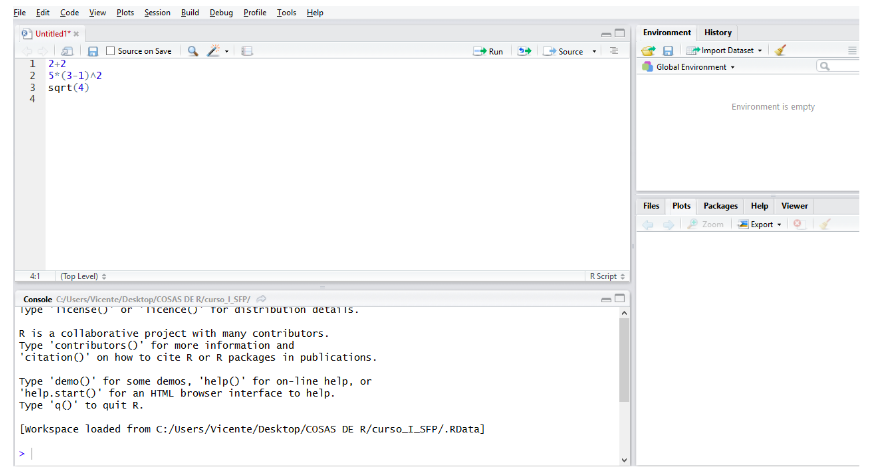
\includegraphics{imagenes/07.png}
Para guardar el script:

\begin{itemize}
\item
  File \textgreater{} Save as.. y seleccionar la ruta donde se quiere guardar el fichero.
\item
  Hacer clic en el botón Guardar que se encuentra en la parte izquierda de la cinta de opciones del script.
\end{itemize}

\hypertarget{entorno}{%
\subsection{Entorno}\label{entorno}}

El panel, llamémoslo, de entorno esta compuesto de dos pestañas: Environment y History.

\begin{itemize}
\tightlist
\item
  En el Environment se irán registrando los objetos que vayamos creando en la sesión de trabajo. También tenemos la opción de cargar y guardar una sesión de trabajo, importar datos y limpiar los objetos de la sesión. Estas opciones están accesibles a través de la cinta de opciones de la pestaña.
\end{itemize}

\begin{figure}
\centering
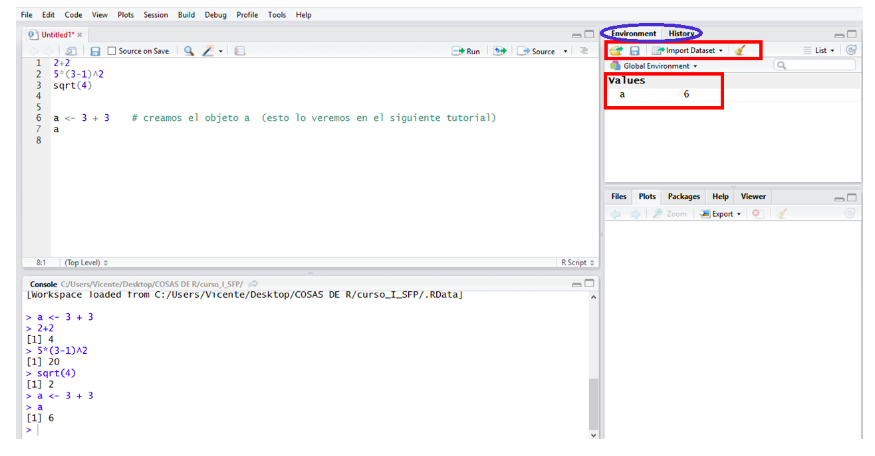
\includegraphics{imagenes/08.png}
\caption{Figura 7}
\end{figure}

\begin{itemize}
\tightlist
\item
  En la pestaña History se registran las instrucciones ejecutadas. Como opciones, podemos cargar y guardar el historial de la sesión, seleccionar una o más instrucciones y enviarlas bien a la consola bien al script, y limpiar el historial.
\end{itemize}

\hypertarget{otros-recursos}{%
\subsection{Otros recursos}\label{otros-recursos}}

Con el nombre de \textbf{Otros recursos} nos referimos al panel que se encuentra en la parte inferior-derecha del escritorio de RStudio. ¡No sabía cómo llamarlo!

En este panel cabe destacar las siguientes pestañas, cada una con diferentes opciones:

\begin{itemize}
\item
  Files: es una especie de explotador de ficheros.
\item
  Plots: donde se visualizan los gráficos que creamos. Entre las opciones disponibles se encuentran:

  \begin{itemize}
  \tightlist
  \item
    Zoom: para agrandar el gráfico y verlo en otra ventana.
  \item
    Export: para exportar/guardar el gráfico. Se puede guardar el gráfico como imagen, pdf o copiarlo al portapapeles.
  \end{itemize}
\item
  Packages: proporciona un listado de los paquetes instalados en R y los que han sido cargado en la sesión. A través de las opciones de esta pestaña podemos instalar nuevos paquetes o actualizar los existentes.
\item
  Help: Para obtener ayuda sobre una determinada función.
\end{itemize}

\hypertarget{configuraciuxf3n-del-espacio-de-trabajo}{%
\section{Configuración del espacio de trabajo}\label{configuraciuxf3n-del-espacio-de-trabajo}}

Antes de comenzar a trabajar debemos fijar el directorio donde queremos guardar nuestros ficheros. Básicamente, dos alternativas.

\hypertarget{opciuxf3n-1-fijar-directorio}{%
\subsection{Opción 1: Fijar directorio}\label{opciuxf3n-1-fijar-directorio}}

Opción 1. Indicamos a R la ruta donde queremos trabajar y la fijamos con la función setwd().

\begin{Shaded}
\begin{Highlighting}[]
\CommentTok{\#setwd("C:/ruta del directorio de trabajo")}
\end{Highlighting}
\end{Shaded}

Para comprobar el directorio de trabajo utilizamos la función getwd():

\begin{Shaded}
\begin{Highlighting}[]
\FunctionTok{getwd}\NormalTok{()}
\end{Highlighting}
\end{Shaded}

\begin{verbatim}
## [1] "/Users/user/Documents/proyectos/capacitacion/capacitacion_R"
\end{verbatim}

Para obtener un listado de los ficheros que contiene la ruta establecida se usa la función dir().

\begin{Shaded}
\begin{Highlighting}[]
\FunctionTok{dir}\NormalTok{()}
\end{Highlighting}
\end{Shaded}

\begin{verbatim}
##  [1] "_book"              "_bookdown_files"    "_bookdown.yml"     
##  [4] "_main_files"        "_main.Rmd"          "_output.yml"       
##  [7] "book.bib"           "capacitacion.Rproj" "css"               
## [10] "data"               "imagenes"           "index.Rmd"         
## [13] "packages.bib"       "preamble.tex"       "README.md"         
## [16] "style.css"
\end{verbatim}

\hypertarget{opciuxf3n-2-proyecto-de-r.}{%
\section{Opción 2 : Proyecto de R.}\label{opciuxf3n-2-proyecto-de-r.}}

Al crear un proyecto todos los ficheros quedan vinculados directamente al proyecto. Para crear un proyecto selección \textbf{File \textgreater{} New project\ldots{}} Se abrirá la siguiente ventana:

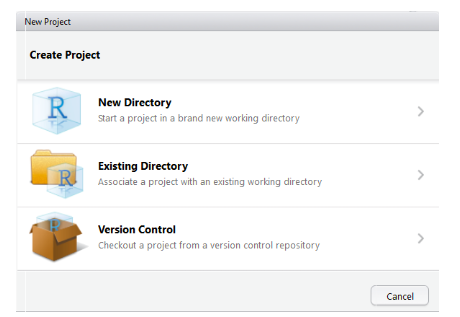
\includegraphics{imagenes/09.png}
Para crear un proyecto en un nuevo directorio, hacemos clic en el botón New Directory. Seguidamente, seleccionamos el tipo de proyecto, en nuestro caso Empty Project. Ahora, asignamos un nombre al directorio (carpeta) que se va a crear y que al mismo tiempo será el nombre del proyecto de R. Para terminar, hacemos clic en el botón Create Project. Al seguir este proceso se habrá creado una carpeta en Documentos y un fichero nombre\_carpeta.Rproj.

Para crear un proyecto en una carpeta que ya existe, hacemos clic en el botón Existing Directory y después seleccionamos la carpeta ayudándonos del Browse.. si fuera necesario. Una vez elegida la carpeta, clicamos en Create Project.

Para abrir un proyecto hacemos doble clic sobre el archivo con extensión .Rproj o lo abrimos desde el menú de RStudio: File \textgreater{} Open Project\ldots{}

Ventaja de los proyectos: cualquier fichero que creemos (script de R, documento de Rmarkdown, etc.) y guardemos se guardará en la carpeta del proyecto.

\hypertarget{instalaciuxf3n-de-paquetes.}{%
\section{Instalación de paquetes.}\label{instalaciuxf3n-de-paquetes.}}

R está compuesto por un sistema base, pero para extender su funcionalidad es necesario instalar paquetes adicionales.

Podemos instalar paquetes de varias formas:

\begin{itemize}
\item
  A través del menú: Tools \textgreater{} Install packages\ldots{}
\item
  En el escritorio de RStudio: Packages/Install. Vemos los paquetes que tenemos actualmente instalados y aquellos que se encuentran cargados.
\end{itemize}

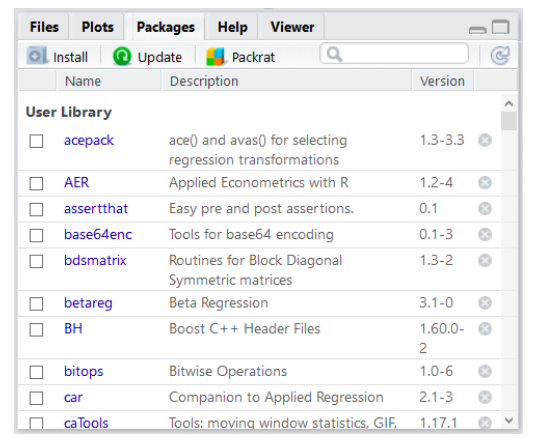
\includegraphics{imagenes/10.png}
- Utilizando la función install.packages(). El nombre del paquete que queremos instalar debe ir entre comillas.

\begin{Shaded}
\begin{Highlighting}[]
\CommentTok{\#install.packages("dplyr") \# dplyr es un paquete que se utiliza para manipular/gestionar datos}
\end{Highlighting}
\end{Shaded}

Una vez instalado el paquete, hay que cargarlo para poderlo utilizar. Esto se hace con la función library().

\begin{Shaded}
\begin{Highlighting}[]
\FunctionTok{library}\NormalTok{(dplyr)}
\end{Highlighting}
\end{Shaded}

\begin{verbatim}
## 
## Attaching package: 'dplyr'
\end{verbatim}

\begin{verbatim}
## The following objects are masked from 'package:stats':
## 
##     filter, lag
\end{verbatim}

\begin{verbatim}
## The following objects are masked from 'package:base':
## 
##     intersect, setdiff, setequal, union
\end{verbatim}

\hypertarget{ayuda-en-r.}{%
\section{Ayuda en R.}\label{ayuda-en-r.}}

En muchas ocasiones necesitamos ayuda sobre cómo funciona una determinada función, cuáles son sus argumentos, etc. Hay varias formas de pedir la ayuda de R. Vamos a pedir la ayuda de la función mean().

\begin{Shaded}
\begin{Highlighting}[]
\FunctionTok{help}\NormalTok{(mean)}
\NormalTok{?mean}
\end{Highlighting}
\end{Shaded}

Si ejecutamos directamente la función library() se abrirá una ventana listando los paquetes que tenemos instalados en R. En el escritorio de RStudio, en la pestaña Packages también tenemos en listado de paquetes instalados (organizados en dos bloques: User Library y System Library)

\begin{Shaded}
\begin{Highlighting}[]
\FunctionTok{library}\NormalTok{()}
\end{Highlighting}
\end{Shaded}

Para obtener ayuda sobre un determinado paquete\ldots{}

\begin{Shaded}
\begin{Highlighting}[]
\FunctionTok{library}\NormalTok{(}\AttributeTok{help=}\StringTok{"foreign"}\NormalTok{)}
\end{Highlighting}
\end{Shaded}

Pero sin duda, una de las mejores fuentes de ayuda en R nos la proporciona internet. Bien haciendo directamente en google la búsqueda sobre el tema que estamos interesados, bien acudiendo a algunas de las muchas webs que ofrecen ayuda. Algunas de las más populares y recomendables webs son:

\begin{itemize}
\item
  \href{https://www.r-bloggers.com/}{R-Bloggers}
\item
  \href{https://stackoverflow.com/}{Stack Overflow}
\end{itemize}

\hypertarget{manipulaciuxf3n-y-visualizaciuxf3n-de-datos}{%
\chapter{Manipulación y visualización de datos}\label{manipulaciuxf3n-y-visualizaciuxf3n-de-datos}}

\hypertarget{comandos-buxe1sicos-de-r.}{%
\section{Comandos básicos de R.}\label{comandos-buxe1sicos-de-r.}}

\hypertarget{introducciuxf3n}{%
\subsection{Introducción}\label{introducciuxf3n}}

El objetivo de este tutorial es familiarizarnos con los conceptos básicos de R. ¿Qué es un objeto en R? ¿Con qué clases/tipos de objetos se trabaja en R?
Aprenderemos a definir vectores y operar con ellos; a crear matrices, listas y data frames; a seleccionar elementos, añadir filas y columnas, etc. Como lo que se pretende es que se entienda la filosofía y la práctica del trabajo con R, todos los conceptos que se introducen se ilustran con ejemplos muy sencillos. No obstante, la selección de funciones que se realiza en este tutorial tienen una aplicación directa en el tratamiento real de datos.

Vamos a realizar paso a paso este sencillo ejercicio para introducir algunos conceptos importantes.

\begin{Shaded}
\begin{Highlighting}[]
\DecValTok{3}\SpecialCharTok{+}\DecValTok{4}
\end{Highlighting}
\end{Shaded}

\begin{verbatim}
## [1] 7
\end{verbatim}

\begin{Shaded}
\begin{Highlighting}[]
\DocumentationTok{\#\# [1] 7}
\FunctionTok{log}\NormalTok{(}\DecValTok{10}\NormalTok{)}
\end{Highlighting}
\end{Shaded}

\begin{verbatim}
## [1] 2.302585
\end{verbatim}

\begin{Shaded}
\begin{Highlighting}[]
\DocumentationTok{\#\# [1] 2.302585}
\NormalTok{x }\OtherTok{\textless{}{-}} \DecValTok{3}\SpecialCharTok{+}\DecValTok{4}  
\NormalTok{x  }\CommentTok{\# x es un vector cuya primera componente es 7. Enseguida vamos con los vectores!}
\end{Highlighting}
\end{Shaded}

\begin{verbatim}
## [1] 7
\end{verbatim}

\begin{Shaded}
\begin{Highlighting}[]
\DocumentationTok{\#\# [1] 7}
\NormalTok{y }\OtherTok{=} \DecValTok{2}\SpecialCharTok{+}\DecValTok{6}
\NormalTok{y}
\end{Highlighting}
\end{Shaded}

\begin{verbatim}
## [1] 8
\end{verbatim}

\begin{Shaded}
\begin{Highlighting}[]
\DocumentationTok{\#\# [1] 8}
\NormalTok{z }\OtherTok{\textless{}{-}} \FunctionTok{c}\NormalTok{(x,y)}
\NormalTok{z}
\end{Highlighting}
\end{Shaded}

\begin{verbatim}
## [1] 7 8
\end{verbatim}

\begin{Shaded}
\begin{Highlighting}[]
\DocumentationTok{\#\# [1] 7 8}
\FunctionTok{mean}\NormalTok{(z)}
\end{Highlighting}
\end{Shaded}

\begin{verbatim}
## [1] 7.5
\end{verbatim}

\begin{Shaded}
\begin{Highlighting}[]
\DocumentationTok{\#\# [1] 7.5}
\NormalTok{w }\OtherTok{\textless{}{-}} \FunctionTok{mean}\NormalTok{(z)}
\NormalTok{w}
\end{Highlighting}
\end{Shaded}

\begin{verbatim}
## [1] 7.5
\end{verbatim}

\begin{Shaded}
\begin{Highlighting}[]
\DocumentationTok{\#\# [1] 7.5}
\FunctionTok{round}\NormalTok{(w, }\AttributeTok{digits=}\DecValTok{0}\NormalTok{)}
\end{Highlighting}
\end{Shaded}

\begin{verbatim}
## [1] 8
\end{verbatim}

\begin{Shaded}
\begin{Highlighting}[]
\DocumentationTok{\#\# [1] 8}
\end{Highlighting}
\end{Shaded}

R utiliza funciones para realizar operaciones. Una función es, por ejemplo, mean(). Para utilizar una función deben especificarse unos argumentos, que es lo que escribimos dentro de los paréntesis. En el caso de la función round() hemos especificado dos argumentos: el vector que queremos redondear (w) y el número de decimales del redondeo (digits).

\textbf{El símbolo \textless- es el operador para asignar. También se puede utilizar = (o menos frecuente -\textgreater), aunque es preferible utilizar el \textless-.}

El símbolo \textbf{\#} se utiliza para introducir un comentario. \textbf{Todo lo que quede a la derecha de \# no se ejecutará.}

Cuando se realiza una asignación se obtiene un objeto. Podemos ver el resultado o contenido de un objeto de varias formas. Por ejemplo, para ver qué es el objeto x podemos escribir en la consola:

\begin{itemize}
\item
  x
\item
  print(x)
\item
  (x \textless- 3+4)
\end{itemize}

\hypertarget{vectores}{%
\subsection{Vectores}\label{vectores}}

Básicamente R trabaja con los siguientes tipos de objetos:

\begin{itemize}
\item
  VECTORES
\item
  MATRICES y ARRAYS (variables indexadas)
\item
  LISTAS
\item
  FACTORES
\item
  DATA FRAMES
\item
  FUNCIONES
\end{itemize}

Empezaremos viendo los objetos más sencillos, los vectores. Poco a poco iremos viendo el resto de objetos.

La mayoría de las operaciones (+, -, *, /) y funciones en R están definidas con carácter vectorial. ¿Qué significa esto? Que R opera componente a componente.

Antes de entender el concepto ``caracter vectorial'', vamos a ver cómo se define/crea un vector.

Para crear un vector se utiliza la función c() (c de concatenate). Por ejemplo:

\begin{Shaded}
\begin{Highlighting}[]
\NormalTok{x }\OtherTok{\textless{}{-}} \FunctionTok{c}\NormalTok{(}\DecValTok{1}\NormalTok{,}\DecValTok{2}\NormalTok{,}\DecValTok{3}\NormalTok{,}\DecValTok{4}\NormalTok{)}
\NormalTok{x                  }\CommentTok{\# x es un vector que tiene cuatro componentes}
\end{Highlighting}
\end{Shaded}

\begin{verbatim}
## [1] 1 2 3 4
\end{verbatim}

\begin{Shaded}
\begin{Highlighting}[]
\NormalTok{y }\OtherTok{\textless{}{-}} \FunctionTok{c}\NormalTok{(}\DecValTok{5}\NormalTok{,}\DecValTok{6}\NormalTok{,}\DecValTok{7}\NormalTok{,}\DecValTok{8}\NormalTok{)}
\NormalTok{y}
\end{Highlighting}
\end{Shaded}

\begin{verbatim}
## [1] 5 6 7 8
\end{verbatim}

Volvemos sobre el tema del carácter vectorial, es decir, se opera componente a componente. Pensemos, si

\begin{Shaded}
\begin{Highlighting}[]
\NormalTok{z }\OtherTok{\textless{}{-}}\NormalTok{ x }\SpecialCharTok{+}\NormalTok{ y}
\end{Highlighting}
\end{Shaded}

¿Qué resultado espero obtener para z?

Exacto!!! Como la operación se realiza vectorialmente (componente a componente, muy importante!) el resultado es:

\begin{Shaded}
\begin{Highlighting}[]
\NormalTok{z}
\end{Highlighting}
\end{Shaded}

\begin{verbatim}
## [1]  6  8 10 12
\end{verbatim}

Vamos a ver si lo entendemos de verdad. Supongamos que x e y son los siguientes vectores:

\begin{Shaded}
\begin{Highlighting}[]
\NormalTok{x }\OtherTok{\textless{}{-}} \FunctionTok{c}\NormalTok{(}\DecValTok{1}\NormalTok{,}\DecValTok{2}\NormalTok{,}\DecValTok{3}\NormalTok{,}\DecValTok{4}\NormalTok{)}
\NormalTok{y }\OtherTok{\textless{}{-}} \FunctionTok{c}\NormalTok{(}\DecValTok{1}\NormalTok{,}\DecValTok{2}\NormalTok{,}\DecValTok{3}\NormalTok{)}
\end{Highlighting}
\end{Shaded}

¿Qué longitud tienen los vectores x e y? Aquí la respuesta está clara, pero en aplicaciones reales utilizaríamos la función length().

\begin{Shaded}
\begin{Highlighting}[]
\FunctionTok{length}\NormalTok{(x)                }\CommentTok{\# esta función es muy útil, conviene recordarla.}
\end{Highlighting}
\end{Shaded}

\begin{verbatim}
## [1] 4
\end{verbatim}

\begin{Shaded}
\begin{Highlighting}[]
\DocumentationTok{\#\# [1] 4}
\FunctionTok{length}\NormalTok{(y)}
\end{Highlighting}
\end{Shaded}

\begin{verbatim}
## [1] 3
\end{verbatim}

\begin{Shaded}
\begin{Highlighting}[]
\DocumentationTok{\#\# [1] 3}
\end{Highlighting}
\end{Shaded}

Los vectores no tienen la misma longitud, entonces.. ¿Cuál será el resultado de z \textless- x + y?

\begin{Shaded}
\begin{Highlighting}[]
\NormalTok{z }\OtherTok{\textless{}{-}}\NormalTok{ x}\SpecialCharTok{+}\NormalTok{y}
\end{Highlighting}
\end{Shaded}

\begin{verbatim}
## Warning in x + y: longer object length is not a multiple of shorter object
## length
\end{verbatim}

\begin{Shaded}
\begin{Highlighting}[]
\NormalTok{z}
\end{Highlighting}
\end{Shaded}

\begin{verbatim}
## [1] 2 4 6 5
\end{verbatim}

R nos da un mensaje de aviso (warning), no es lo mismo que un error. Nos avisa que hay algo que no cuadra pero\ldots realiza la operación que nosotros queremos.

Una cuestión muy importante que siempre tenemos que tener en cuenta cuando trabajamos con vectores es que en un vector sólo podemos concatenar elementos del mismo tipo. ¿Qué tipos/clases de elementos (o datos) tenemos en R?

\begin{itemize}
\item
  Carácter
\item
  Numéricos
\item
  Enteros
\item
  Complejos
\item
  Lógicos
\end{itemize}

Veamos algunos ejemplos\ldots{}

\begin{Shaded}
\begin{Highlighting}[]
\NormalTok{x }\OtherTok{\textless{}{-}} \FunctionTok{c}\NormalTok{(}\DecValTok{1}\NormalTok{,}\DecValTok{2}\NormalTok{,}\DecValTok{3}\NormalTok{,}\DecValTok{4}\NormalTok{)    }\CommentTok{\# creamos el vector x}
\FunctionTok{class}\NormalTok{(x)           }\CommentTok{\# devuelve el tipo de objeto}
\end{Highlighting}
\end{Shaded}

\begin{verbatim}
## [1] "numeric"
\end{verbatim}

\begin{Shaded}
\begin{Highlighting}[]
\NormalTok{y }\OtherTok{\textless{}{-}} \FunctionTok{c}\NormalTok{(}\StringTok{"a"}\NormalTok{,}\StringTok{"b"}\NormalTok{)}
\FunctionTok{class}\NormalTok{(y)}
\end{Highlighting}
\end{Shaded}

\begin{verbatim}
## [1] "character"
\end{verbatim}

\begin{Shaded}
\begin{Highlighting}[]
\NormalTok{z }\OtherTok{\textless{}{-}} \FunctionTok{c}\NormalTok{(1L,2L,3L)   }\CommentTok{\# escribimos L detrás del número para obligar a que sea entero}
\FunctionTok{class}\NormalTok{(z)}
\end{Highlighting}
\end{Shaded}

\begin{verbatim}
## [1] "integer"
\end{verbatim}

\begin{Shaded}
\begin{Highlighting}[]
\NormalTok{w }\OtherTok{\textless{}{-}} \FunctionTok{c}\NormalTok{(}\ConstantTok{TRUE}\NormalTok{, F)    }\CommentTok{\# en general, puede escribirse TRUE/FALSE o T/F}
\FunctionTok{class}\NormalTok{(w)}
\end{Highlighting}
\end{Shaded}

\begin{verbatim}
## [1] "logical"
\end{verbatim}

\begin{Shaded}
\begin{Highlighting}[]
\NormalTok{t }\OtherTok{\textless{}{-}} \FunctionTok{c}\NormalTok{(}\DecValTok{1}\SpecialCharTok{+}\NormalTok{2i, }\DecValTok{1}\SpecialCharTok{+}\NormalTok{3i)}
\FunctionTok{class}\NormalTok{(t)}
\end{Highlighting}
\end{Shaded}

\begin{verbatim}
## [1] "complex"
\end{verbatim}

En los ejemplos anteriores hemos definido un vector en el que todos sus elementos eran del mismo tipo. Pero\ldots.¿qué pasa si tenemos los siguientes vectores?

\begin{Shaded}
\begin{Highlighting}[]
\NormalTok{x }\OtherTok{\textless{}{-}} \FunctionTok{c}\NormalTok{(}\DecValTok{1}\NormalTok{,}\DecValTok{2}\NormalTok{,}\StringTok{"a"}\NormalTok{)}
\NormalTok{y }\OtherTok{\textless{}{-}} \FunctionTok{c}\NormalTok{(}\ConstantTok{FALSE}\NormalTok{, }\DecValTok{1}\NormalTok{)}
\NormalTok{z }\OtherTok{\textless{}{-}} \FunctionTok{c}\NormalTok{(}\StringTok{"a"}\NormalTok{,T)}
\end{Highlighting}
\end{Shaded}

¿De qué tipo son ahora los vectores x, y, z?

\begin{Shaded}
\begin{Highlighting}[]
\FunctionTok{class}\NormalTok{(x)}
\end{Highlighting}
\end{Shaded}

\begin{verbatim}
## [1] "character"
\end{verbatim}

\begin{Shaded}
\begin{Highlighting}[]
\DocumentationTok{\#\# [1] "character"}
\FunctionTok{class}\NormalTok{(y)}
\end{Highlighting}
\end{Shaded}

\begin{verbatim}
## [1] "numeric"
\end{verbatim}

\begin{Shaded}
\begin{Highlighting}[]
\DocumentationTok{\#\# [1] "numeric"}
\FunctionTok{class}\NormalTok{(z)}
\end{Highlighting}
\end{Shaded}

\begin{verbatim}
## [1] "character"
\end{verbatim}

\begin{Shaded}
\begin{Highlighting}[]
\DocumentationTok{\#\# [1] "character"}
\end{Highlighting}
\end{Shaded}

R ha forzado a que todos los elementos del vector sean del mismo tipo. A esto se le llama implicit coercion. Fijémonos cúal es el resultado de los vectores que hemos definido antes.

\begin{Shaded}
\begin{Highlighting}[]
\NormalTok{x}
\end{Highlighting}
\end{Shaded}

\begin{verbatim}
## [1] "1" "2" "a"
\end{verbatim}

\begin{Shaded}
\begin{Highlighting}[]
\NormalTok{y}
\end{Highlighting}
\end{Shaded}

\begin{verbatim}
## [1] 0 1
\end{verbatim}

\begin{Shaded}
\begin{Highlighting}[]
\NormalTok{z}
\end{Highlighting}
\end{Shaded}

\begin{verbatim}
## [1] "a"    "TRUE"
\end{verbatim}

En ocasiones somos nosotros los que estamos interesados en forzar que todos los elementos del vector sean del mismo tipo (esto es la explicit coercion). Para ello utilizamos las funciones as.numeric() , as.character(), as.logical() \ldots{} Si el resultado no tiene sentido R producirá un mensaje de error o warning. Un ejemplo:

\begin{Shaded}
\begin{Highlighting}[]
\NormalTok{x }\OtherTok{\textless{}{-}} \FunctionTok{c}\NormalTok{(}\DecValTok{1}\NormalTok{,}\DecValTok{2}\NormalTok{,}\StringTok{"a"}\NormalTok{)}
\NormalTok{x}
\end{Highlighting}
\end{Shaded}

\begin{verbatim}
## [1] "1" "2" "a"
\end{verbatim}

\begin{Shaded}
\begin{Highlighting}[]
\DocumentationTok{\#\# [1] "1" "2" "a"}
\FunctionTok{as.numeric}\NormalTok{(x)}
\end{Highlighting}
\end{Shaded}

\begin{verbatim}
## Warning: NAs introduced by coercion
\end{verbatim}

\begin{verbatim}
## [1]  1  2 NA
\end{verbatim}

\begin{Shaded}
\begin{Highlighting}[]
\DocumentationTok{\#\# [1]  1  2 NA}
\FunctionTok{as.character}\NormalTok{(x)}
\end{Highlighting}
\end{Shaded}

\begin{verbatim}
## [1] "1" "2" "a"
\end{verbatim}

\begin{Shaded}
\begin{Highlighting}[]
\DocumentationTok{\#\# [1] "1" "2" "a"}
\end{Highlighting}
\end{Shaded}

Por último, podemos evaluar el tipo/clase de objeto con las funciones is.numeric(), is.character(), etc.

\hypertarget{acceder-a-un-elemento-de-un-objeto}{%
\subsubsection{Acceder a un elemento de un objeto}\label{acceder-a-un-elemento-de-un-objeto}}

Para seleccionar/acceder a un elemento de un objeto se suelen emplear: \textbf{{[}{]}, \$, {[}{[}{]}{]}.}

Vamos a crear el objeto x que será un vector de cuatro componentes formado por los cuatro primeros números pares. Así:

\begin{Shaded}
\begin{Highlighting}[]
\NormalTok{x }\OtherTok{\textless{}{-}} \FunctionTok{c}\NormalTok{(}\DecValTok{2}\NormalTok{,}\DecValTok{4}\NormalTok{,}\DecValTok{6}\NormalTok{,}\DecValTok{8}\NormalTok{)}
\end{Highlighting}
\end{Shaded}

Si queremos acceder/seleccionar/extraer al/el segundo componente de x

\begin{Shaded}
\begin{Highlighting}[]
\NormalTok{x[}\DecValTok{2}\NormalTok{]}
\end{Highlighting}
\end{Shaded}

\begin{verbatim}
## [1] 4
\end{verbatim}

\hypertarget{enlistar-y-borrar-objetos}{%
\subsubsection{Enlistar y borrar objetos}\label{enlistar-y-borrar-objetos}}

Las funciones ls() y objects() hacen lo mismo: listan los objetos que hemos definido en la sesión.

\begin{Shaded}
\begin{Highlighting}[]
\FunctionTok{ls}\NormalTok{()}
\end{Highlighting}
\end{Shaded}

\begin{verbatim}
## [1] "t" "w" "x" "y" "z"
\end{verbatim}

\begin{Shaded}
\begin{Highlighting}[]
\FunctionTok{objects}\NormalTok{()}
\end{Highlighting}
\end{Shaded}

\begin{verbatim}
## [1] "t" "w" "x" "y" "z"
\end{verbatim}

Si queremos borrar objetos utilizamos la función rm()

\begin{Shaded}
\begin{Highlighting}[]
\FunctionTok{rm}\NormalTok{(z)  }\CommentTok{\# borramos el objeto z}
\FunctionTok{ls}\NormalTok{()}
\end{Highlighting}
\end{Shaded}

\begin{verbatim}
## [1] "t" "w" "x" "y"
\end{verbatim}

y si estamos interesados en borrar todos los objetos que hemos definido:

\begin{Shaded}
\begin{Highlighting}[]
\FunctionTok{rm}\NormalTok{(}\AttributeTok{list=}\FunctionTok{ls}\NormalTok{()) }\CommentTok{\# o también rm(list=objects())}
\FunctionTok{ls}\NormalTok{()}
\end{Highlighting}
\end{Shaded}

\begin{verbatim}
## character(0)
\end{verbatim}

\hypertarget{tipos-de-objetos}{%
\subsection{Tipos de objetos}\label{tipos-de-objetos}}

\hypertarget{matrices}{%
\subsubsection{Matrices}\label{matrices}}

La función matrix() permite organizar los datos en una matriz con tantas filas y columnas como se indiquen.

Vamos a pedir ayuda a R sobre la función matrix()

\begin{Shaded}
\begin{Highlighting}[]
\NormalTok{?matrix }\CommentTok{\# una forma de obtener ayuda en R es escribiendo ? delante de la función de la que solicitamos ayuda}
\end{Highlighting}
\end{Shaded}

\hypertarget{cuxf3mo-crear-y-trabajar-con-matrices}{%
\paragraph{Cómo crear y trabajar con matrices}\label{cuxf3mo-crear-y-trabajar-con-matrices}}

Una vez hemos leído en la ayuda cómo usar la función matrix, vamos a practicarlo con el siguiente ejemplo. Pero antes de ejecutarlo, pensemos en qué es lo que queremos hacer y, sobre todo, pensemos en cuál es el resultado que esperamos obtener.

\begin{Shaded}
\begin{Highlighting}[]
\NormalTok{x }\OtherTok{\textless{}{-}} \FunctionTok{matrix}\NormalTok{ (}\AttributeTok{data=} \FunctionTok{c}\NormalTok{(}\DecValTok{1}\NormalTok{,}\DecValTok{2}\NormalTok{,}\DecValTok{3}\NormalTok{,}\DecValTok{4}\NormalTok{), }\AttributeTok{nrow=}\DecValTok{2}\NormalTok{, }\AttributeTok{ncol=}\DecValTok{2}\NormalTok{) }\CommentTok{\# o x \textless{}{-} matrix (c(1,2,3,4), nrow=2, ncol=2)}
\NormalTok{x}
\end{Highlighting}
\end{Shaded}

\begin{verbatim}
##      [,1] [,2]
## [1,]    1    3
## [2,]    2    4
\end{verbatim}

Observemos que se ha creado una matrix de 2x2 (2 filas y 2 columnas) y, además, muy importante, ¿cómo se ha completado la matriz? ¡Exacto! La matriz se ha rellenado por columnas. Si queremos que se rellene por filas hay que incluir el argumento byrow en los argumentos de la función.

\begin{Shaded}
\begin{Highlighting}[]
\NormalTok{y }\OtherTok{\textless{}{-}} \FunctionTok{matrix}\NormalTok{ (}\FunctionTok{c}\NormalTok{(}\DecValTok{1}\NormalTok{,}\DecValTok{2}\NormalTok{,}\DecValTok{3}\NormalTok{,}\DecValTok{4}\NormalTok{), }\AttributeTok{nrow=}\DecValTok{2}\NormalTok{, }\AttributeTok{ncol=}\DecValTok{2}\NormalTok{, }\AttributeTok{byrow=}\NormalTok{T)}
\NormalTok{y}
\end{Highlighting}
\end{Shaded}

\begin{verbatim}
##      [,1] [,2]
## [1,]    1    2
## [2,]    3    4
\end{verbatim}

Fíjense en la diferencia entre los objetos x e y.

Una forma más simple para definir una matrix es:

\begin{Shaded}
\begin{Highlighting}[]
\NormalTok{y }\OtherTok{\textless{}{-}} \FunctionTok{matrix}\NormalTok{ (}\FunctionTok{c}\NormalTok{(}\DecValTok{1}\NormalTok{,}\DecValTok{2}\NormalTok{,}\DecValTok{3}\NormalTok{,}\DecValTok{4}\NormalTok{), }\DecValTok{2}\NormalTok{, }\DecValTok{2}\NormalTok{, }\AttributeTok{byrow=}\NormalTok{T)}
\NormalTok{y}
\end{Highlighting}
\end{Shaded}

\begin{verbatim}
##      [,1] [,2]
## [1,]    1    2
## [2,]    3    4
\end{verbatim}

aunque también podíamos haber omitido el argumento relativo al número de filas o de columnas, porque conocida una dimensión R completaría la matrix dados los datos con los que se trabaja.

\begin{Shaded}
\begin{Highlighting}[]
\NormalTok{y }\OtherTok{\textless{}{-}} \FunctionTok{matrix}\NormalTok{ (}\FunctionTok{c}\NormalTok{(}\DecValTok{1}\NormalTok{,}\DecValTok{2}\NormalTok{,}\DecValTok{3}\NormalTok{,}\DecValTok{4}\NormalTok{), }\DecValTok{2}\NormalTok{, }\AttributeTok{byrow=}\NormalTok{T)  }\CommentTok{\# no especificamos nrow porque por defecto es el primer argumento después de los datos}
\NormalTok{y}
\end{Highlighting}
\end{Shaded}

\begin{verbatim}
##      [,1] [,2]
## [1,]    1    2
## [2,]    3    4
\end{verbatim}

\begin{Shaded}
\begin{Highlighting}[]
\NormalTok{x }\OtherTok{\textless{}{-}} \FunctionTok{matrix}\NormalTok{(}\FunctionTok{c}\NormalTok{(}\DecValTok{1}\NormalTok{,}\DecValTok{2}\NormalTok{,}\DecValTok{3}\NormalTok{,}\DecValTok{4}\NormalTok{,}\DecValTok{5}\NormalTok{,}\DecValTok{6}\NormalTok{), }\AttributeTok{ncol=}\DecValTok{3}\NormalTok{)}
\NormalTok{x}
\end{Highlighting}
\end{Shaded}

\begin{verbatim}
##      [,1] [,2] [,3]
## [1,]    1    3    5
## [2,]    2    4    6
\end{verbatim}

\hypertarget{seleccionando-elementos-de-una-matriz}{%
\subsubsection{Seleccionando elementos de una matriz}\label{seleccionando-elementos-de-una-matriz}}

Lo primero, vamos a crear el objeto A que será una matriz.

\begin{Shaded}
\begin{Highlighting}[]
\NormalTok{A }\OtherTok{\textless{}{-}} \FunctionTok{matrix}\NormalTok{(}\DecValTok{1}\SpecialCharTok{:}\DecValTok{16}\NormalTok{,}\DecValTok{4}\NormalTok{,}\DecValTok{4}\NormalTok{)}
\NormalTok{A}
\end{Highlighting}
\end{Shaded}

\begin{verbatim}
##      [,1] [,2] [,3] [,4]
## [1,]    1    5    9   13
## [2,]    2    6   10   14
## [3,]    3    7   11   15
## [4,]    4    8   12   16
\end{verbatim}

Para seleccionar elementos de una matriz utilizamos el símbolo de los corchetes: {[}{]}.

Pensemos un momento en el posible resultado de estos ejemplos antes de efectuarlos.

\begin{Shaded}
\begin{Highlighting}[]
\NormalTok{A[}\DecValTok{2}\NormalTok{,}\DecValTok{3}\NormalTok{]}
\end{Highlighting}
\end{Shaded}

\begin{verbatim}
## [1] 10
\end{verbatim}

\begin{Shaded}
\begin{Highlighting}[]
\NormalTok{A[}\FunctionTok{c}\NormalTok{(}\DecValTok{1}\NormalTok{,}\DecValTok{2}\NormalTok{),}\FunctionTok{c}\NormalTok{(}\DecValTok{2}\NormalTok{,}\DecValTok{4}\NormalTok{)]}
\end{Highlighting}
\end{Shaded}

\begin{verbatim}
##      [,1] [,2]
## [1,]    5   13
## [2,]    6   14
\end{verbatim}

\begin{Shaded}
\begin{Highlighting}[]
\NormalTok{A[}\DecValTok{1}\SpecialCharTok{:}\DecValTok{3}\NormalTok{,}\DecValTok{2}\SpecialCharTok{:}\DecValTok{4}\NormalTok{]}
\end{Highlighting}
\end{Shaded}

\begin{verbatim}
##      [,1] [,2] [,3]
## [1,]    5    9   13
## [2,]    6   10   14
## [3,]    7   11   15
\end{verbatim}

\begin{Shaded}
\begin{Highlighting}[]
\NormalTok{A[}\DecValTok{1}\NormalTok{,]}
\end{Highlighting}
\end{Shaded}

\begin{verbatim}
## [1]  1  5  9 13
\end{verbatim}

\begin{Shaded}
\begin{Highlighting}[]
\NormalTok{A[}\DecValTok{1}\SpecialCharTok{:}\DecValTok{2}\NormalTok{,]}
\end{Highlighting}
\end{Shaded}

\begin{verbatim}
##      [,1] [,2] [,3] [,4]
## [1,]    1    5    9   13
## [2,]    2    6   10   14
\end{verbatim}

\begin{Shaded}
\begin{Highlighting}[]
\NormalTok{A[,}\DecValTok{2}\SpecialCharTok{:}\DecValTok{3}\NormalTok{]}
\end{Highlighting}
\end{Shaded}

\begin{verbatim}
##      [,1] [,2]
## [1,]    5    9
## [2,]    6   10
## [3,]    7   11
## [4,]    8   12
\end{verbatim}

\hypertarget{listas}{%
\subsection{Listas}\label{listas}}

A diferencia de los vectores o matrices, las listas pueden contener elementos/componentes de distinto tipo. Observemos esta lista que tiene 5 componentes (pueden ser matrices, vectores, dataframes,..).

\begin{Shaded}
\begin{Highlighting}[]
\NormalTok{x }\OtherTok{\textless{}{-}} \FunctionTok{list}\NormalTok{(}\FunctionTok{c}\NormalTok{(}\DecValTok{1}\NormalTok{,}\DecValTok{2}\NormalTok{,}\DecValTok{3}\NormalTok{,}\DecValTok{4}\NormalTok{), }\StringTok{"Curso"}\NormalTok{, F, }\DecValTok{1}\SpecialCharTok{+}\NormalTok{2i, 3L,A)}
\NormalTok{x}
\end{Highlighting}
\end{Shaded}

\begin{verbatim}
## [[1]]
## [1] 1 2 3 4
## 
## [[2]]
## [1] "Curso"
## 
## [[3]]
## [1] FALSE
## 
## [[4]]
## [1] 1+2i
## 
## [[5]]
## [1] 3
## 
## [[6]]
##      [,1] [,2] [,3] [,4]
## [1,]    1    5    9   13
## [2,]    2    6   10   14
## [3,]    3    7   11   15
## [4,]    4    8   12   16
\end{verbatim}

Utilizamos el doble corchete {[}{[}{]}{]} para acceder al contenido concreto de una lista.

\begin{Shaded}
\begin{Highlighting}[]
\NormalTok{x[[}\DecValTok{3}\NormalTok{]]  }\CommentTok{\# accedemos al tercer componente de la lista}
\end{Highlighting}
\end{Shaded}

\begin{verbatim}
## [1] FALSE
\end{verbatim}

\begin{Shaded}
\begin{Highlighting}[]
\NormalTok{x[[}\DecValTok{1}\NormalTok{]][}\DecValTok{2}\NormalTok{] }\CommentTok{\# accedemos al segundo elemento del primer componente de la lista}
\end{Highlighting}
\end{Shaded}

\begin{verbatim}
## [1] 2
\end{verbatim}

\begin{Shaded}
\begin{Highlighting}[]
\NormalTok{x[[}\DecValTok{6}\NormalTok{]][}\DecValTok{1}\NormalTok{,}\DecValTok{2}\NormalTok{]}
\end{Highlighting}
\end{Shaded}

\begin{verbatim}
## [1] 5
\end{verbatim}

Vamos a crear otra lista para practicar.

\begin{Shaded}
\begin{Highlighting}[]
\NormalTok{y }\OtherTok{\textless{}{-}} \FunctionTok{list}\NormalTok{( }\AttributeTok{Titulacion =} \FunctionTok{c}\NormalTok{(}\StringTok{"Economía"}\NormalTok{, }\StringTok{"Sociología"}\NormalTok{, }\StringTok{"Derecho"}\NormalTok{), }\AttributeTok{Edad =}\FunctionTok{c}\NormalTok{(}\DecValTok{25}\NormalTok{,}\DecValTok{26}\NormalTok{,}\DecValTok{27}\NormalTok{))}

\NormalTok{y}
\end{Highlighting}
\end{Shaded}

\begin{verbatim}
## $Titulacion
## [1] "Economía"   "Sociología" "Derecho"   
## 
## $Edad
## [1] 25 26 27
\end{verbatim}

Fijémonos en la diferencia de presentación de las listas x e y. Como en la lista y hemos nombrado los componentes, estos aparecen al ejecutar el objeto precedidos del símbolo \$. Ahora también podemos acceder a un componente de la lista por su nombre.

\begin{Shaded}
\begin{Highlighting}[]
\NormalTok{y}\SpecialCharTok{$}\NormalTok{Titulacion}
\end{Highlighting}
\end{Shaded}

\begin{verbatim}
## [1] "Economía"   "Sociología" "Derecho"
\end{verbatim}

\begin{Shaded}
\begin{Highlighting}[]
\NormalTok{y[[}\DecValTok{1}\NormalTok{]]}
\end{Highlighting}
\end{Shaded}

\begin{verbatim}
## [1] "Economía"   "Sociología" "Derecho"
\end{verbatim}

Evidentemente, también podemos realizar operaciones con listas.

\begin{Shaded}
\begin{Highlighting}[]
\NormalTok{y[[}\DecValTok{2}\NormalTok{]]}\SpecialCharTok{*}\DecValTok{3}
\end{Highlighting}
\end{Shaded}

\begin{verbatim}
## [1] 75 78 81
\end{verbatim}

\hypertarget{data-frame}{%
\subsection{Data Frame}\label{data-frame}}

Los data frame se usan para almacenar datos en forma de tablas (filas / columnas), como estamos habituados en Excel, Spss, etc.

Los data frame pueden almacenar objetos/datos de distinto tipo: numéricos, carácter, \ldots{} En las matrices todos los elementos tenían que ser enteros o numéricos.

Los data frame pueden entenderse como un tipo especial de lista donde cada elemento de la lista tiene que tener la misma longitud. Cada elemento de la lista sería una columna y la longitud de cada elemento de la lista serían las filas.

\textbf{Aunque normalmente los data frame los creamos al cargar/leer una base de datos (ver el tutorial), vamos crear una data frame para ver su estructura.}

\begin{Shaded}
\begin{Highlighting}[]
\NormalTok{x }\OtherTok{\textless{}{-}} \FunctionTok{data.frame}\NormalTok{(}\AttributeTok{Titulacion =} \FunctionTok{c}\NormalTok{(}\StringTok{"Economía"}\NormalTok{, }\StringTok{"ADE"}\NormalTok{, }\StringTok{"Sociología"}\NormalTok{, }\StringTok{"Magisterio"}\NormalTok{), }\AttributeTok{Edad =} \FunctionTok{c}\NormalTok{(}\DecValTok{25}\NormalTok{, }\DecValTok{27}\NormalTok{, }\DecValTok{25}\NormalTok{, }\DecValTok{24}\NormalTok{))}
\NormalTok{x}
\end{Highlighting}
\end{Shaded}

\begin{verbatim}
##   Titulacion Edad
## 1   Economía   25
## 2        ADE   27
## 3 Sociología   25
## 4 Magisterio   24
\end{verbatim}

\hypertarget{importar-y-exportar-datos}{%
\subsection{Importar y exportar datos}\label{importar-y-exportar-datos}}

\hypertarget{manipulaciuxf3n-y-limpieza-de-datos.}{%
\section{Manipulación y limpieza de datos.}\label{manipulaciuxf3n-y-limpieza-de-datos.}}

  \bibliography{book.bib,packages.bib}

\end{document}
